\chapter{A titulação}\label{ch:g11:titration}

A caixa de um suplemento de ferro promete \qty{80}{mg} de ferro em cada
comprimido, na forma de \omterm{def:g9:ions:ion}{íons} ferro(II). Será verdade? Um químico tritura
um comprimido, dissolve-o em ácido e acrescenta, gota a gota, uma
solução violeta de permanganato de potássio a partir de um longo tubo
graduado. Cada gota perde a cor na hora, à medida que os \omterm{def:g9:ions:ion}{íons}
permanganato são consumidos pelos \omterm{def:g9:ions:ion}{íons} ferro(II), até que uma gota, a
última, deixa um rosa claro que não desaparece. O volume despejado nesse
momento dá a quantidade de ferro. Este capítulo transforma uma reação
numa medida.

\begin{recall}
Um \omterm{def:g11:redox:oxidant}{oxidante} ganha \omterm{def:g9:inside-the-atom:nucleus}{elétrons}, um \omterm{def:g11:redox:oxidant}{redutor} os cede; o \omterm{def:g9:ions:ion}{íon} permanganato oxida
os \omterm{def:g9:ions:ion}{íons} ferro(II) segundo
\ce{MnO4^- + 8H+ + 5Fe^{2+} -> Mn^{2+} + 5Fe^{3+} + 4H2O}
(\cref{ch:g11:redox}). A \omterm{def:g10:concentration-and-dilution:molar-concentration}{concentração molar} e a \omterm{def:g10:concentration-and-dilution:dilution}{diluição}
(\cref{ch:g10:concentration-and-dilution}); a \omterm{def:g10:reaction-progress-table:extent}{tabela de avanço} e o
\omterm{def:g10:reaction-progress-table:limiting}{reagente limitante} (\cref{ch:g10:reaction-progress-table}).
\end{recall}

\begin{omfigure}
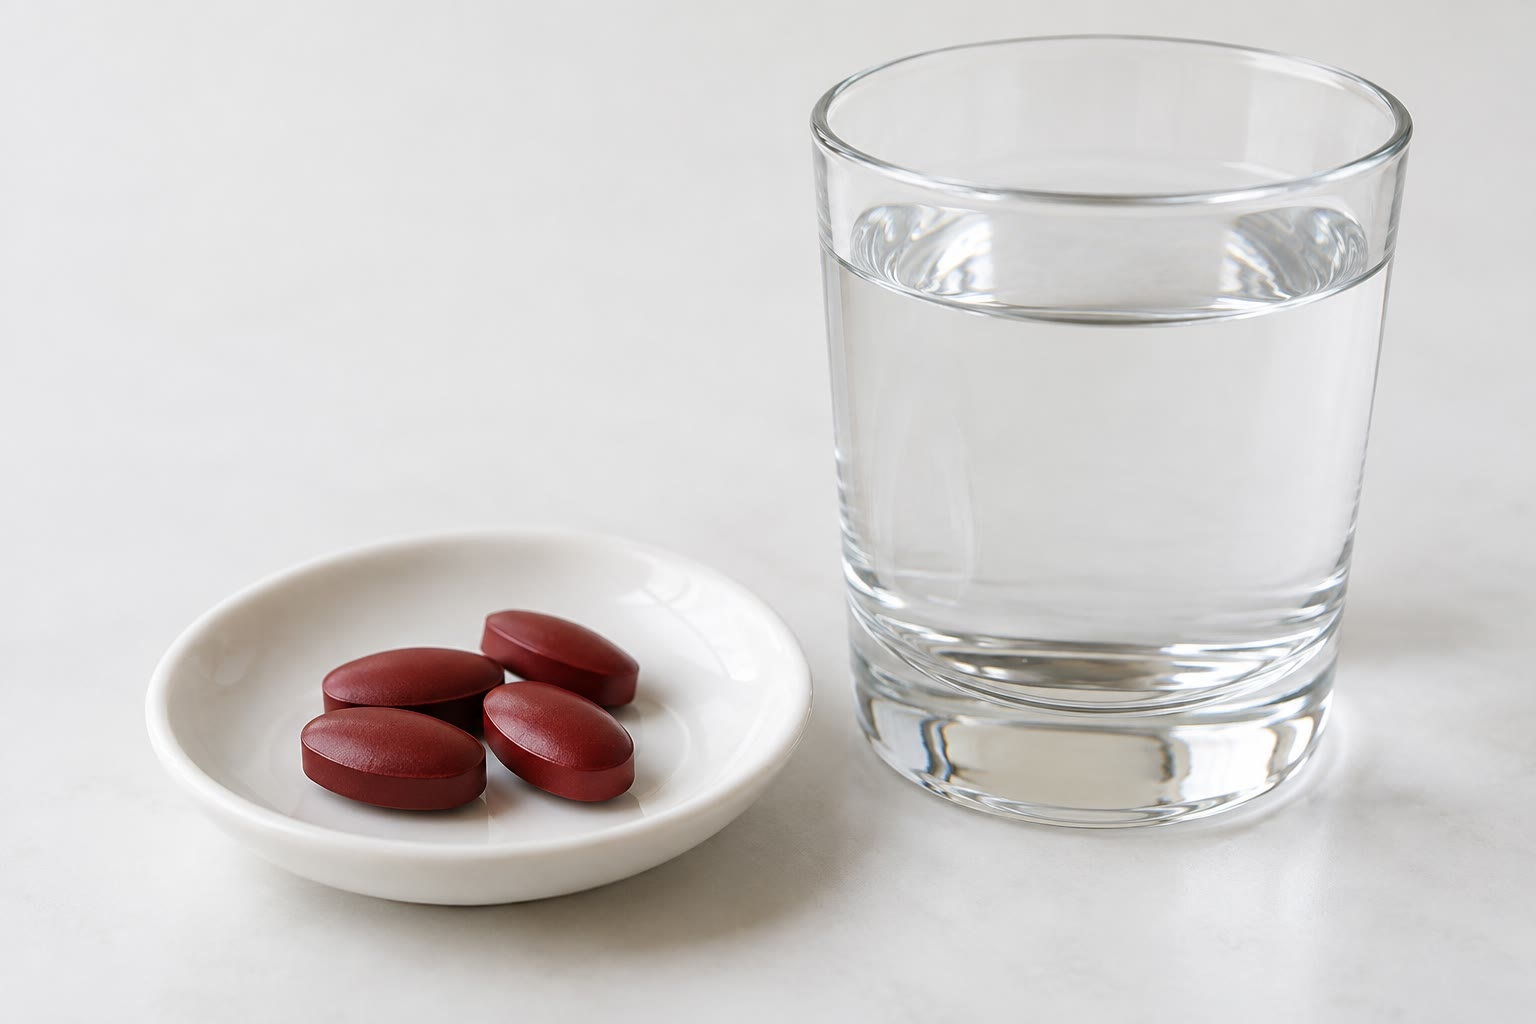
\includegraphics[width=0.45\linewidth]{images/book1/ai/g11-iron-tablets.jpg}

{\small Comprimidos de suplemento de ferro: quanto ferro cada um contém
de verdade?}
\end{omfigure}

\section{Titular}

\begin{definition}[Titulação, titulante, solução titulada]\label{def:g11:titration:titration}
Uma \emph{titulação}\index{titulacao@titulação} mede a quantidade de uma espécie
dissolvida fazendo-a reagir com outra espécie cuja concentração é
conhecida com exatidão. A solução de concentração conhecida, acrescentada
a partir de uma bureta, é o \emph{titulante}\index{titulante}; a solução
que contém a espécie a medir, colocada no frasco, é a \emph{solução
titulada}\index{solucao titulada@solução titulada}.
\end{definition}

\begin{proposition}[Como deve ser uma reação de titulação]\label{prop:g11:titration:conditions}
Uma reação pode ser usada numa \omterm{def:g11:titration:titration}{titulação} se ela for total (para que um
\omterm{def:g7:chemical-reactions:reactant}{reagente} se esgote inteiramente), rápida (para que cada gota reaja na
hora) e única (o \omterm{def:g11:titration:titration}{titulante} não reage com mais nada no frasco).
\end{proposition}

\begin{proof}
Se a reação parasse antes de terminar, ficasse atrasada em relação às
gotas ou consumisse \omterm{def:g11:titration:titration}{titulante} em outra coisa, o volume despejado não
mediria mais a quantidade da espécie titulada.
\end{proof}

\begin{omfigure}
\begin{tikzpicture}[font=\small, scale=0.62]
  \pic[transform shape] at (0,0) {stand={5.8}{1.8}};
  \pic[transform shape] at (1.8,0.68) {stirrer};
  \pic[transform shape] at (1.8,0.68) {erlenmeyer={0.25}{yellow!12}};
  \pic[transform shape] at (1.8,2.98) {burette={0.75}{violet!55}};
  \draw[omProp, thick, <-] (2.15,6.9) -- (4.2,7.4) node[right, text=black,
    align=left] {bureta: titulante\\ (permanganato de potássio)};
  \draw[omProp, thick, <-] (2.55,1.4) -- (4.2,1.9) node[right, text=black,
    align=left] {erlenmeyer: solução\\ titulada (ferro(II), ácido)};
  \draw[omProp, thick, <-] (3.0,0.4) -- (4.2,0.3) node[right, text=black]
    {agitador magnético};
\end{tikzpicture}

{\small Uma montagem de \omterm{def:g11:titration:titration}{titulação}: a bureta, presa a um suporte, fornece
o \omterm{def:g11:titration:titration}{titulante} à \omterm{def:g11:titration:titration}{solução titulada}, mantida sob agitação.}
\end{omfigure}

\section{A equivalência}

\begin{definition}[Equivalência, volume de equivalência]\label{def:g11:titration:equivalence}
A \emph{equivalência}\index{equivalencia@equivalência} é o momento de uma \omterm{def:g11:titration:titration}{titulação}
em que o \omterm{def:g11:titration:titration}{titulante} acrescentado e a espécie titulada estão nas
proporções da equação: os dois estão consumidos. O volume de \omterm{def:g11:titration:titration}{titulante}
despejado nesse momento é o
\emph{volume de equivalência}\index{volume de equivalencia@volume de equivalência}, $V_E$.
\end{definition}

\begin{proposition}[A relação na equivalência]\label{prop:g11:titration:relation}
Para uma reação de \omterm{def:g11:titration:titration}{titulação} $a\,\ce{A} + b\,\ce{B} \longrightarrow$ produtos, com A titulado (quantidade
$n_A$) por um \omterm{def:g11:titration:titration}{titulante} B de concentração $c_B$, na \omterm{def:g11:titration:equivalence}{equivalência}
\[
  \frac{n_A}{a} = \frac{c_B\, V_E}{b} .
\]
\end{proposition}

\begin{proof}
Na \omterm{def:g11:titration:equivalence}{equivalência}, a \omterm{def:g6:pure-substances-and-mixtures:mixture}{mistura} é estequiométrica
(\cref{ch:g10:reaction-progress-table}): A e B, de quantidades iniciais
$n_A$
e $c_B V_E$, se esgotam juntos, logo $n_A / a = c_B V_E / b$.
\end{proof}

\begin{omfigure}
\begin{tikzpicture}
\begin{axis}[width=0.72\linewidth, height=5.6cm, xmin=0, xmax=20,
    ymin=0, ymax=16, xlabel={volume de titulante acrescentado (\si{mL})},
    ylabel={quantidade ($\num{e-4}$ \si{mol})}, axis lines*=left, ymajorgrids,
    grid style={gray!20}, tick label style={font=\small},
    label style={font=\small}, legend style={font=\small, at={(0.98,0.97)},
    anchor=north east, draw=none}, legend cell align=left]
  \addplot[very thick, orange!70!black, domain=0:14.3] {14.3 - x};
  \addplot[very thick, violet, domain=14.3:20] {0.2*(x - 14.3)};
  \addplot[very thick, violet, domain=0:14.3, forget plot] {0};
  \legend{\ce{Fe^{2+}} que resta no frasco, \ce{MnO4^-} em excesso}
  \addplot[dashed, black!60] coordinates {(14.3,0) (14.3,7)};
  \node[font=\small, anchor=west] at (axis cs:14.5,6.5) {$V_E = \qty{14.3}{mL}$};
\end{axis}
\end{tikzpicture}

{\small Ferro(II) titulado pelo permanganato a \qty{0.0200}{mol/L}: os
\omterm{def:g9:ions:ion}{íons} ferro(II) se esgotam exatamente no \omterm{def:g11:titration:equivalence}{volume de equivalência}; depois
dele, os \omterm{def:g9:ions:ion}{íons} permanganato não são mais consumidos e se acumulam.}
\end{omfigure}

\section{Localizar a equivalência por uma mudança de cor}


\begin{proposition}[Ver a equivalência]\label{prop:g11:titration:colour}
Quando uma das espécies da \omterm{def:g11:titration:titration}{titulação} é colorida, a \omterm{def:g11:titration:equivalence}{equivalência} é vista
como uma mudança de cor do frasco: a cor do \omterm{def:g11:titration:titration}{titulante} aparece e persiste
assim que o \omterm{def:g11:titration:titration}{titulante} está em excesso, ou a cor da espécie titulada
desaparece quando ela se esgota.
\end{proposition}

\begin{proof}
Antes da \omterm{def:g11:titration:equivalence}{equivalência}, cada \omterm{def:g9:ions:ion}{íon} de \omterm{def:g11:titration:titration}{titulante} que cai no frasco é
consumido na hora; depois da \omterm{def:g11:titration:equivalence}{equivalência}, ele permanece. Uma espécie
colorida só está presente no frasco, portanto, de um lado da
\omterm{def:g11:titration:equivalence}{equivalência}.
\end{proof}

\begin{example}[O permanganato, o seu próprio indicador]\label{ex:g11:titration:permanganate}
O \omterm{def:g9:ions:ion}{íon} permanganato \ce{MnO4^-} é violeta intenso, e os \omterm{def:g9:ions:ion}{íons} manganês
\ce{Mn^{2+}} que ele dá são quase incolores; os \omterm{def:g9:ions:ion}{íons} ferro só dão à
solução uma leve tonalidade amarela. Antes da \omterm{def:g11:titration:equivalence}{equivalência}, cada gota
violeta é descorada ao cair; a primeira gota que não é descorada marca a
\omterm{def:g11:titration:equivalence}{equivalência}: o frasco fica rosa claro e continua assim.
\end{example}

\begin{omfigure}
\begin{tikzpicture}[font=\small]
  \pic at (0,0) {erlenmeyer={0.3}{yellow!14}};
  \pic at (3.2,0) {erlenmeyer={0.3}{magenta!10}};
  \pic at (6.4,0) {erlenmeyer={0.3}{violet!45}};
  \node[align=center, anchor=north] at (0,-0.15) {antes da equivalência:\\
    amarelo claro, cada gota\\ descorada};
  \node[align=center, anchor=north] at (3.2,-0.15) {na equivalência:\\
    um rosa claro que\\ persiste};
  \node[align=center, anchor=north] at (6.4,-0.15) {depois da equivalência:\\
    violeta (permanganato\\ em excesso)};
\end{tikzpicture}

{\small O frasco de uma \omterm{def:g11:titration:titration}{titulação} de ferro(II) pelo permanganato, antes,
na e depois da \omterm{def:g11:titration:equivalence}{equivalência}. O \omterm{def:g11:titration:equivalence}{volume de equivalência} é lido no primeiro
rosa que persiste.}
\end{omfigure}

\begin{example}[A vitamina C e o iodo]\label{ex:g11:titration:vitamin-c}
% ledger: aw:C, aw:H, aw:O
A vitamina C, o ácido ascórbico \ce{C6H8O6} ($M = \qty{176.0}{g/mol}$), é
um \omterm{def:g11:redox:oxidant}{redutor}; o iodo \ce{I2} a oxida:
\[
  \ce{C6H8O6 + I2 -> C6H6O6 + 2H+ + 2I-} .
\]
\qty{10.0}{mL} de suco de laranja, com um pouco de amido, são titulados
por uma solução de iodo a \qty{5.00e-3}{mol/L}. Antes da \omterm{def:g11:titration:equivalence}{equivalência}, o
iodo é consumido; a primeira gota em excesso deixa o amido azul-escuro.
Se $V_E = \qty{5.70}{mL}$, o suco continha
$n = \num{5.00e-3} \times \num{5.70e-3} = \qty{2.85e-5}{mol}$ de vitamina
C, isto é, \qty{5.0}{mg} em \qty{10.0}{mL}: \qty{0.50}{g/L}.
\end{example}

\section{Calcular uma concentração desconhecida}

\begin{method}[Calcular uma concentração a partir de uma titulação]\label{met:g11:titration:computing}
\begin{enumerate}
  \item Escreva a \omterm{def:g8:balanced-equations:equation}{equação balanceada} da reação de \omterm{def:g11:titration:titration}{titulação} e leia os
        coeficientes $a$ (espécie titulada) e $b$ (\omterm{def:g11:titration:titration}{titulante}).
  \item Leia $V_E$ na bureta, e calcule a quantidade de \omterm{def:g11:titration:titration}{titulante}
        despejada, $n_B = c_B V_E$.
  \item Na \omterm{def:g11:titration:equivalence}{equivalência}, $n_A = \dfrac{a}{b}\, c_B V_E$.
  \item Divida pelo volume titulado: $c_A = n_A / V_A$. Se a amostra foi
        diluída antes da \omterm{def:g11:titration:titration}{titulação}, multiplique pelo \omterm{def:g10:concentration-and-dilution:dilution}{fator de diluição}.
\end{enumerate}
\end{method}

\begin{example}[Uma solução de ferro(II)]\label{ex:g11:titration:iron}
\qty{20.0}{mL} de uma solução de ferro(II), acidificada, precisam de
$V_E = \qty{12.6}{mL}$ de permanganato a \qty{0.0200}{mol/L}. Aqui
$a = 5$ (\ce{Fe^{2+}}) e $b = 1$ (\ce{MnO4^-}):
$n(\ce{MnO4^-}) = 0.0200 \times 0.0126 = \qty{2.52e-4}{mol}$, logo
$n(\ce{Fe^{2+}}) = 5 \times \num{2.52e-4} = \qty{1.26e-3}{mol}$, e
$c(\ce{Fe^{2+}}) = \num{1.26e-3} / 0.0200 = \qty{0.0630}{mol/L}$.
\end{example}

\section{A titulação como medida}

\begin{inthelab}[Ler uma bureta]
A bureta é enxaguada com o \omterm{def:g11:titration:titration}{titulante}, enchida, e a sua ponta é livrada
das bolhas de \omterm{def:g4:air-a-mixture-of-gases:air}{ar}. O nível é lido na parte de baixo do menisco, com o
olho na mesma altura, antes e depois da \omterm{def:g11:titration:titration}{titulação}: o volume despejado é
a diferença. As graduações são de \qty{0.1}{mL} em \qty{0.1}{mL}, e uma
leitura pode ser estimada a \qty{0.05}{mL}. Perto da \omterm{def:g11:titration:equivalence}{equivalência}, o
\omterm{def:g11:titration:titration}{titulante} é acrescentado gota a gota, enquanto o frasco é agitado.
\end{inthelab}

\begin{omfigure}
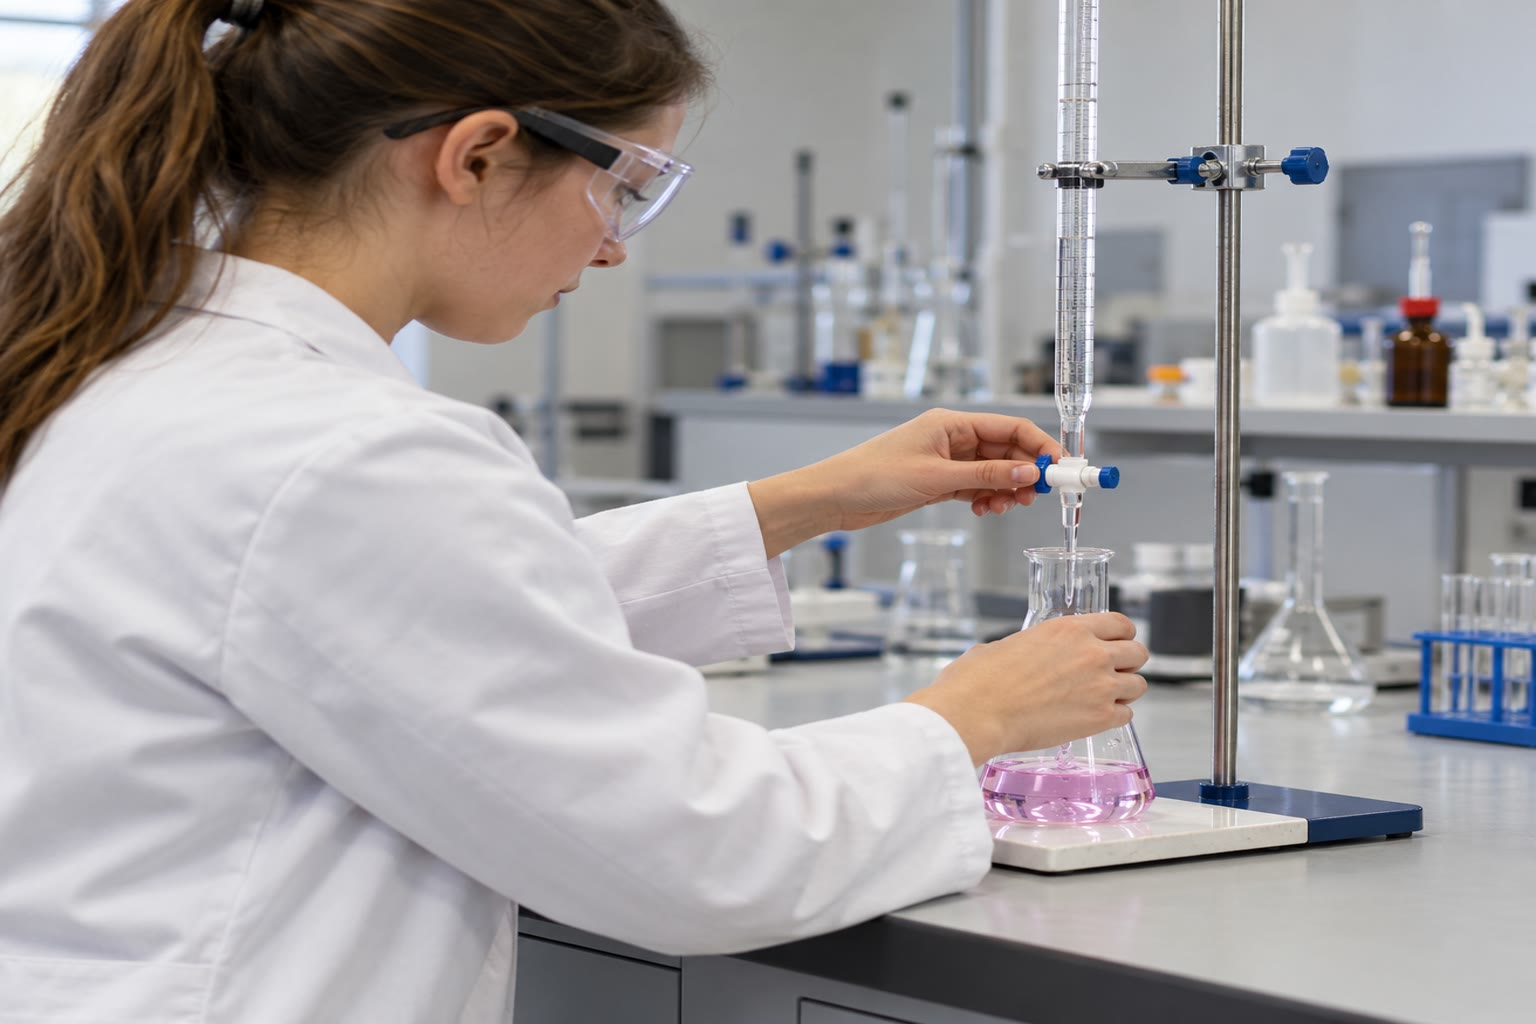
\includegraphics[width=0.48\linewidth]{images/book1/ai/g11-titration-bench.jpg}

{\small Uma \omterm{def:g11:titration:titration}{titulação} em andamento: bureta, suporte e erlenmeyer sobre
um azulejo branco.}
\end{omfigure}

\begin{remark}[Qual é a precisão de uma titulação?]\label{rem:g11:titration:precision}
Cada leitura da bureta pode errar em cerca de \qty{0.05}{mL}, e o volume
despejado é a diferença de duas leituras: pode errar em até
\qty{0.1}{mL}. Para $V_E = \qty{14.3}{mL}$, isso dá $0.1 / 14.3 \approx
\qty{0.7}{\percent}$. Um $V_E$ maior torna esse erro relativo menor, e é
por isso que as concentrações dos \omterm{def:g11:titration:titration}{titulantes} são escolhidas para dar
\omterm{def:g11:titration:equivalence}{volumes de equivalência} de 10 a \qty{20}{mL} com uma bureta de
\qty{25}{mL}. A \omterm{def:g11:titration:titration}{titulação} é repetida até que dois resultados concordem
dentro de cerca de \qty{0.1}{mL}. Um tratamento mais fino da incerteza
de uma medida é dado no volume do primeiro ano da universidade.
\end{remark}

\begin{safety}{\ghs[0.7cm]{GHS03}\ghs[0.7cm]{GHS05}\ghs[0.7cm]{GHS07}\ghs[0.7cm]{GHS08}\ghs[0.7cm]{GHS09}}
% ledger: ghs:KMnO4, ghs:I2
O permanganato de potássio sólido é um \omterm{def:g11:redox:oxidant}{oxidante} que pode alimentar um
incêndio, corrosivo e nocivo; as suas soluções diluídas mancham de
marrom a pele e as roupas. As soluções de iodo são nocivas. Óculos de
proteção e luvas; os resíduos são recolhidos, nunca jogados na pia.
\end{safety}

\section{Exercícios}


\begin{exercise}[$\star$]\label{exo:g11:titration:1}
Numa \omterm{def:g11:titration:titration}{titulação}, o que é o \omterm{def:g11:titration:titration}{titulante}? E a \omterm{def:g11:titration:titration}{solução titulada}? O que
acontece na \omterm{def:g11:titration:equivalence}{equivalência}?
\end{exercise}

\begin{exercise}[$\star$]\label{exo:g11:titration:2}
Que quantidade de \omterm{def:g9:ions:ion}{íons} permanganato está contida em \qty{12.5}{mL} de
uma solução a \qty{0.0200}{mol/L}?
\end{exercise}

\begin{exercise}[$\star$]\label{exo:g11:titration:3}
Na figura das quantidades em função do volume despejado, leia o \omterm{def:g11:titration:equivalence}{volume
de equivalência}. Que quantidade de ferro(II) havia no frasco no início?
\end{exercise}

\begin{exercise}[$\star$]\label{exo:g11:titration:4}
Por que não é preciso indicador numa \omterm{def:g11:titration:titration}{titulação} pelo permanganato?
\end{exercise}

\begin{exercise}[$\star$]\label{exo:g11:titration:5}
Na \omterm{def:g11:titration:equivalence}{equivalência} da \omterm{def:g11:titration:titration}{titulação} do ferro(II) pelo permanganato, qual é a
razão entre a quantidade de ferro(II) e a quantidade de permanganato
despejada? Por quê?
\end{exercise}

\begin{exercise}[$\star\star$]\label{exo:g11:titration:6}
\qty{10.0}{mL} de uma solução acidificada de ferro(II) precisam de
\qty{8.40}{mL} de permanganato a \qty{0.0200}{mol/L}. Calcule a
\omterm{def:g10:concentration-and-dilution:molar-concentration}{concentração molar} do ferro(II), e depois a sua \omterm{def:g10:concentration-and-dilution:mass-concentration}{concentração em massa}.
\end{exercise}

\begin{exercise}[$\star\star$]\label{exo:g11:titration:7}
Um comprimido de vitamina C é dissolvido para fazer \qty{100.0}{mL} de
solução. \qty{10.0}{mL} dela, com amido, precisam de \qty{11.4}{mL} de
iodo a \qty{0.0100}{mol/L}. Que massa de vitamina C o comprimido
contém?
\end{exercise}

\begin{exercise}[$\star\star$]\label{exo:g11:titration:8}
Uma reação é total, mas leva vários minutos. Por que ela não pode ser
usada assim numa \omterm{def:g11:titration:titration}{titulação} com mudança de cor?
\end{exercise}

\begin{exercise}[$\star\star$]\label{exo:g11:titration:9}
Olhe os três frascos. Uma aluna para num frasco tão violeta quanto o
terceiro. O \omterm{def:g11:titration:equivalence}{volume de equivalência} dela é grande ou pequeno demais? O
que ela deveria ter feito perto da \omterm{def:g11:titration:equivalence}{equivalência}?
\end{exercise}

\begin{exercise}[$\star\star$]\label{exo:g11:titration:10}
Uma solução concentrada de ferro(II) é primeiro diluída dez vezes.
Depois, \qty{10.0}{mL} da solução diluída precisam de \qty{13.0}{mL} de
permanganato a \qty{0.0200}{mol/L}. Encontre a concentração da solução
concentrada.
\end{exercise}

\begin{exercise}[$\star\star$]\label{exo:g11:titration:11}
% ledger: aw:Fe
A solução de ferro(II) do exemplo resolvido do capítulo tem
$c = \qty{0.0630}{mol/L}$. Que massa de ferro contém \qty{1.00}{L}
dela?
\end{exercise}

\begin{exercise}[$\star\star\star$]\label{exo:g11:titration:12}
Uma \omterm{def:g11:titration:titration}{titulação} dá $V_E = \qty{7.2}{mL}$. Estime o erro relativo devido às
leituras da bureta, e compare com $V_E = \qty{14.3}{mL}$. Sugira duas
maneiras de obter um \omterm{def:g11:titration:equivalence}{volume de equivalência} maior.
\end{exercise}

\begin{exercise}[$\star\star\star$]\label{exo:g11:titration:13}
O peróxido de hidrogênio é titulado pelo permanganato em meio ácido:
\[
  \ce{2MnO4^- + 5H2O2 + 6H+ -> 2Mn^{2+} + 5O2 + 8H2O} .
\]
Um desinfetante é diluído dez vezes; \qty{10.0}{mL} da solução diluída
precisam de \qty{17.6}{mL} de permanganato a \qty{0.0200}{mol/L}.
Encontre a \omterm{def:g10:concentration-and-dilution:molar-concentration}{concentração molar} de peróxido de hidrogênio no desinfetante,
e depois a sua \omterm{def:g10:concentration-and-dilution:mass-concentration}{concentração em massa} (\ce{H2O2}: \qty{34.0}{g/mol}).
\end{exercise}

\begin{exercise}[$\star\star\star$]\label{exo:g11:titration:14}
Um comprimido de ferro deveria conter cerca de \qty{1.4e-3}{mol} de
ferro(II). Que concentração de permanganato dá um \omterm{def:g11:titration:equivalence}{volume de equivalência}
perto de \qty{15}{mL} com uma bureta de \qty{25}{mL}? O que daria errado
com uma solução dez vezes mais concentrada?
\end{exercise}

\begin{exercise}[$\star\star\star$]\label{exo:g11:titration:15}
A equação da \omterm{def:g11:titration:titration}{titulação} mostra \ce{8H+} para cada \ce{MnO4^-}. Para um
\omterm{def:g11:titration:equivalence}{volume de equivalência} de \qty{14.3}{mL} a \qty{0.0200}{mol/L}, que
quantidade de \omterm{def:g9:ions:ion}{íons} hidrogênio é consumida? \qty{10}{mL} de um ácido com
\qty{1.0}{mol/L} de \omterm{def:g9:ions:ion}{íons} hidrogênio bastam? Por que o frasco deve ser
acidificado?
\end{exercise}

\section{Problema: o comprimido de ferro é honesto?}

\begin{problem}[{Problema de fim de semana --- um suplemento de ferro
anuncia 80 mg de ferro por comprimido: uma titulação concorda?}]
\label{pb:g11:titration:1}
% ledger: aw:Fe, aw:S, aw:O, const:NA
A caixa de um suplemento de ferro anuncia \qty{80}{mg} de ferro, na
forma de ferro(II), por comprimido. Um comprimido é triturado e
dissolvido em cerca de \qty{50}{mL} de ácido sulfúrico diluído, e depois
titulado pelo permanganato de potássio a \qty{0.0200}{mol/L}. O rosa
claro persiste em $V_E = \qty{14.3}{mL}$.

\medskip
\noindent\textbf{Parte I --- A reação.}
\begin{enumerate}
  \item Dê o nome dos dois \omterm{def:g11:redox:couple}{pares redox} envolvidos. Que espécie é o
        \omterm{def:g11:redox:oxidant}{oxidante}, e qual é o \omterm{def:g11:redox:oxidant}{redutor}?
  \item Escreva as duas \omterm{def:g11:redox:couple}{semirreações}.
  \item Combine-as na equação da \omterm{def:g11:titration:titration}{titulação}, e verifique que ela está
        balanceada em carga.
  \item Por que o comprimido é dissolvido em ácido?
  \item Mostre que a reação cumpre as condições de uma \omterm{def:g11:titration:titration}{titulação}, e
        explique como a \omterm{def:g11:titration:equivalence}{equivalência} é vista.
\end{enumerate}

\medskip
\noindent\textbf{Parte II --- A \omterm{def:g11:titration:titration}{titulação}.}
\begin{enumerate}[resume]
  \item Em que vidraria fica a solução de permanganato? Como o seu
        volume é lido?
  \item De que cor é o frasco antes da \omterm{def:g11:titration:equivalence}{equivalência}, e por que cada gota
        perde a cor?
  \item Calcule a quantidade de permanganato despejada na \omterm{def:g11:titration:equivalence}{equivalência}.
\end{enumerate}

\medskip
\noindent\textbf{Parte III --- O ferro.}
\begin{enumerate}[resume]
  \item Deduza a quantidade de ferro(II) do comprimido.
  \item Calcule a sua massa em miligramas.
  \item Compare com o rótulo: qual é a diferença relativa?
  \item O volume despejado pode errar em \qty{0.1}{mL}. Em quantos
        miligramas a massa de ferro pode errar? O rótulo é confirmado?
\end{enumerate}

\medskip
\noindent\textbf{Parte IV --- Vários comprimidos.}
\begin{enumerate}[resume]
  \item Outros dois comprimidos dão $V_E = \qty{14.1}{mL}$ e
        \qty{14.4}{mL}. Calcule as suas massas de ferro.
  \item Calcule a média dos três comprimidos.
  \item Os três resultados diferem mais do que o erro da bureta. O que
        isso diz sobre os comprimidos?
  \item Um permanganato a \qty{0.100}{mol/L} teria sido uma escolha
        melhor? Explique.
  \item Muitos suplementos também contêm vitamina C, um \omterm{def:g11:redox:oxidant}{redutor}. O que
        ela faria com a \omterm{def:g11:titration:titration}{titulação}, e com a massa de ferro encontrada?
  \item O ferro está presente como sulfato de ferro(II), \ce{FeSO4}. Que
        massa dele um comprimido contém?
  \item Quantos \omterm{def:g9:ions:ion}{íons} ferro(II) isso representa?
  \item Dê a resposta final: que massa de ferro um comprimido contém?
\end{enumerate}
\end{problem}
